% !TEX TS-program = xelatex
% !TEX encoding = UTF-8

\documentclass[11pt,a4paper,draft]{article} 
\usepackage[a4paper,margin=0pt,left=0mm]{geometry}
\usepackage[T1]{fontenc} 
\usepackage{times,graphicx}
\usepackage[grid=false,subgridcolor=green!20,	% grid used only in draft mode
                   gridcolor=gray!80, texcoord=true, 
                   gridunit=cm]{eso-pic}
%\defaultfontfeatures{Mapping=tex-text} 
%\usepackage{xunicode} 
%\usepackage{xltxtra} 
%\usepackage{geometry}
\usepackage{times}
\usepackage{xcolor,rotating}
\usepackage{graphicx} 
\makeatletter
\newif\if@debug
\fboxsep0pt
\fboxrule0pt
\@debugfalse
\if@debug
   \def\rulecolor{gray}%
   \fboxsep-0.2pt 
  \fboxrule0.2pt
\else
  \fboxsep0pt
  \fboxrule0pt
\fi
\parskip0pt
%\def\includegraphics#1{\expandafter\@gobble{#1}\rule{100pt}{50pt}}
% first block mitteilungen
  \def\A{\fbox{
\includegraphics{img-01}}}
  \def\B{\fbox{
\includegraphics{img-02}}}
  \def\C{\fbox{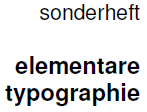
\includegraphics{img-03}}}
  \def\D{\fbox{
\includegraphics{img-04}}}
  \def\E{\fbox{
\includegraphics{img-05}}}
  \def\offsetXY#1#2#3{\hskip#1\raise#2\vbox{\hbox{#3}}}
  \def\offsetY#1{\vspace*{#1}}
  \def\offsetrule#1#2{ \color{\rulecolor}\rule{#1}{#2}}
\parindent0pt
\begin{document}
\makeatletter
\topskip0pt
\parindent0pt
\newlength\xgrid
\newlength\ygrid
\def\hopx#1{\hspace*{#1\xgrid\relax}}
\def\hopy#1{\vspace*{#1\ygrid\relax}}
\setlength\xgrid{54.15pt} % this is possibly correct
\setlength\ygrid{20mm}   % this not sure does not look right
\def\rulei {{\color{red}\rule{5.7in}{1pc}}}
\def\ruleii {{\color{red}\rule{1pc}{23.5cm}}}
\def\ruleiii{{\color{black}\rule{152pt}{10pt}}}


\def\C{\hspace*{\dimexpr\xgrid-7pt}\turnbox{90}{\fbox{\fontsize{52}{50}\sffamily\bfseries \hspace{9mm} phase 3a \& phase 3b}}}




\newbox\AAA
\setbox\AAA\hbox{%
{\fontsize{52}{50}\sffamily\bfseries \fbox{\hbox to 5.7in{\hfill city center}}}}


\expandafter\protected@xdef\csname AAA@wd\endcsname{\the\wd\AAA}
%  \the\dp\AAA\\
%  \the\ht\AAA\\

% Mitteilungen
\hopy{2}
\vskip3pt

\hspace*{20pt}\rulei\vskip3pt
\hspace*{20pt}\unhbox\AAA\par

% Vertical red stripe

\hspace*{10mm}\vbox to 23.5cm{\fbox{\hbox to \dimexpr 2\xgrid{\hfill\ruleii}}}%

% add typographie
\vspace*{-4.35cm}\hskip2\xgrid\hskip10mm\C 

\vspace{-13.52cm}
\hopx{4}\hspace{4mm}
\fbox{\parbox{180pt}
                 {\raggedleft
                         \fontsize{28}{20}\sffamily March 2012
                         \vspace{1cm}

                         \fontsize{31}{36}\sffamily\bfseries 
                         MEP\\ Interim Progress Report}}

\vspace*{.5in}
\hopx{7.5}
\fbox{\parbox{140pt}
                 {\raggedright \fontsize{13}{14}\sffamily\bfseries 
                       {\Large{HLS}\includegraphics[scale=0.2]{specon-logo-02} }
                       \vspace{1.2\baselineskip}\\
                       Yiannis Lazarides \\
                       Nidhal Hammadi \\
                       Shadi Alashkar \\
                       Rabieh Wehbe\\
                       George Georgiou\\
                      \vspace{3.8\baselineskip}
                       }}

\def\ccc {\fontsize{12}{10}\sffamily 
                      \quad zeitschrift des bildungsverbandes der
                      deutschen buchdrucker leipzig 
                     \textbullet{} oktoberheft 1925}

\let\div\hbox%
%\vspace*{-25.4cm}
\hopy{-12.6}
\hopx{10}\hspace*{15pt}
 \div{\hbox to 23.5cm{{\turnbox{-90}{\fbox{\div{\ccc\kern 3cm\ruleiii}}}}}}

\fboxrule1pt

\def\ZZZ{\fbox{\begin{minipage}[b]{100pt}{\vspace{30pt}This is some text and this is some other
\vspace{50pt}
}\end{minipage}}}



\newcommand{\ZZ}[1][]{\fbox{\begin{minipage}[b]{100pt}{\vspace{0pt} \hspace*{1cm}\vbox{This is some text and this is some other\par}

 \vtop{\rule{1pt}{#1}}
}\end{minipage}}}

\newpage

\vspace*{5cm}

\ZZ[9cm]\hbox to 100pt{\ZZ[11cm]{\ZZZ\ZZZ}}\ZZ[8cm]\ruleii 

\end{document}

@YiannisLazarides the titlepage of "elementare typographie" is slightly larger than my scanner so there is perhaps one 1cm missing at the bottom dl.dropbox.com/u/55981144/…
@YiannisLazarides I also added a the inner title page which is also interesting I guess. The left margin should equal the right margin, but this was difficult to scan so it got cropped on the left. Notice the placement of "oktoberheft 1925" which seems to be aligned on the x-height. dl.dropbox.com/u/55981144/… .... happy griding ;-)
  
 

Yiannis Lazarides
@FrankMittelbach Thanks a lot.

@FrankMittelbach They look ok, if it is not too much trouble can you measure the pages. I have used a4 so far as you did, but I had a lot of trouble with a grid, especially at the first vertical line, so maybe this explains it. Vertical grid so far on title page seems to be 54pt but probably was 3/4 of inch.

elementare-typographie sizes:

left margin to red line = 8pc
top margin to red line = 11.5pc

horizonal redline = 1pc x 39pc starting at left margin
vertical red line = 1 pc x 56.5pc from bottom

page width = 55pc
page height = 73,5pc






